\documentclass{sciposter}
\usepackage{lipsum}
\usepackage{epsfig}
\usepackage{amsmath}
\usepackage{amssymb}
\usepackage{multicol}
\usepackage{graphicx,url}
\usepackage[portuges, brazil]{babel}   
\usepackage[utf8]{inputenc}
%\usepackage{fancybullets}
\newtheorem{Def}{Definition}


\title{Classifying hot water chemistry: 
\\ Application of multivariate statistics}
%Título do projeto

\author{Prihadi Sumintadireja, Dasapta Erwin Irawan, Rina Herdianita, Yuano Rezky, Prana Ugiana Gio, Anggita Agustin}
%nome dos autores

\institute 
{Faculty of Earth Sciences and Technology, Institut Teknologi Bandung \\
Ministry of Energy and Mineral Resources of Indonesia \\
Faculty of Math and Natural Sciences, Universitas Sumatera Utara}
%Nome e endereço da Instituição

\email{dasaptaerwin@outlook.co.id}

%\date is unused by the current \maketitle

\rightlogo[1]{logo_usu_esdm.jpg}
\leftlogo[1]{logo_itb.jpg}
% Exibe os logos (direita e esquerda) 
% Procure usar arquivos png ou jpg, e de preferencia mantenha na mesma pasta do .tex
%%%%%%%%%%%%%%%%%%%%%%%%%%%%%%%%%%%%%%%%%%%%%%%%%%%%%%%%%%%%%%%%%%%%%%%%%%%%%%%%
%%% Begin of Document



\begin{document}
%define conference poster is presented at (appears as footer)

\conference{{\bf LPPM ITB Research Poster Expo 2016}, CRCS ITB, 21 December 2016}

%\LEFTSIDEfootlogo  
% Uncomment to put footer logo on left side, and 
% conference name on right side of footer

% Some examples of caption control (remove % to check result)

%\renewcommand{\algorithmname}{Algoritme} % for Dutch

%\renewcommand{\mastercapstartstyle}[1]{\textit{\textbf{#1}}}
%\renewcommand{\algcapstartstyle}[1]{\textsc{\textbf{#1}}}
%\renewcommand{\algcapbodystyle}{\bfseries}
%\renewcommand{\thealgorithm}{\Roman{algorithm}}

\maketitle

%%% Begin of Multicols-Enviroment
\begin{multicols}{3}

%%% Abstract
\begin{abstract}
The following paper is a try out on the application of multivariate analysis (regression tree, principal component analysis, and cluster analysis) for classifying hot water chemistry. The number of sample analysed was 416 from all over Indonesia. Regression tree technique has failed to read the data structure due to multi-collinearity effect therefore PCA and cluster analysis were applied.  We used open source R statistical packages to do the calculation. Such technique classifies hot water samples into three major clusters: cluster 1 (pure hot water), cluster 2 (mixing water), and cluster 3 (cold-meteoric water). Similar clustering were also detected in the PCA plot. The statistical is able to detect the close and open geothermal system based on data structure. This robust method should be applied to more geothermal system with larger dataset to see its performance. 

\end{abstract}

%%% Introduction
\section{Introduction}
Indonesia ranked 3rd in the world in both geothermal electricity production and geothermal generating capacity in 2014. Our current geothermal capacity of 1.3 GW consists of plants clustered around Java, Bali, North Sumatra, and North Sulawesi (Bronto, 2006; Darmawan et al., 2015; Fauzi, 2015; Manalu, 1988; Smillie et al., n.d.). However, despite of the various techniques used in geothermal exploration, the application of multivariate analysis/statistics is still very low (Agustin et al., 2015). Such large quantity of measured parameters in each observation site needs to be deeply analysed using a robust multivariate technique. This paper is one of our methodological trial offering correlations between statistical and deterministic model. 

\section{Materials and method}
\subsection{Data}
The data was gathered from various sources: EBTKE reports, researches from ITB and other universities. At least 30 variables were measured on each samples (Table 1).

\begin{table}[]
\centering
\caption{The description of variables in the dataset}
\label{descriptor}
\begin{tabular}{llll}
No & Parameters & Parameters           & Units            \\
1  & elv        & elevation            & masl             \\
2  & wtemp      & water temperature    & oC               \\
3  & atemp      & air temperature      & oC               \\
4  & ph         & pH                   & -                \\
5  & ec         & Electro Conductivity & mikroSiemens/cm \\
6  & SiO2       & Silica               & mg/L             \\
7  & B          & Boron                & mg/L             \\
8  & Al         & Aluminium            & mg/L             \\
9  & Fe         & Iron                 & mg/L             \\
10 & Ca         & Calsium              & mg/L             \\
11 & Mg         & Magnesium            & mg/L             \\
12 & Na         & Sodium               & mg/L             \\
13 & K          & Potassium            & mg/L             \\
14 & Li         & Lithium              & mg/L             \\
15 & As         & Arsen                & mg/L             \\
16 & NH4        & Amonium              & mg/L             \\
17 & F          & Fluor                & mg/L             \\
18 & Cl         & Chlor                & mg/L             \\
19 & SO4        & Sulfate              & mg/L             \\
20 & HCO3       & Bicarbonate          & mg/L            
\end{tabular}
\end{table}

\subsection{Software and code}
To ensure the reproducibility of this work and to support open science principals, we made the code and dataset available on OSF server (https://osf.io/wbnz3/). We used R statistical program and R Studio. It is open source and can be downloaded from (https://cran.r-project.org and http://rstudio.com), along with some add on packages.

\subsection{Regression tree method}
Regression tree mainly uses the principal of linear model. It is one of the most frequently used machine-learning methods for building prediction models. As a result, the partitioning can be represented graphically as a decision tree (ath and Fabricius, 2000; Faraway, 2005; Gio, Prana Ugiana and Rosmaini, Elly, 2015; Gregor et al., 2002; Loh, 2011; Rothwell et al., 2008). Relying on the assumption of normal distribution and no collinearity within the dataset, we expect the method could split the samples into several classes (Kuhn, 2008; Lewis, 2000).

\subsection{Cluster analysis and principal component analysis}
Cluster analysis (CA) is an unsupervised classification method of a set of objects in groups. The HCA is useful for variables or observations, categorical data, or continuous variables. Principal component analysis (PCA) is another form of unsupervised classification method applying the rotation of covariance matrix to reduce the dimension of the dataset by retaining most of the information in the original set (Chen et al., 2007; Fitzpatrick et al., 2007; Irawan et al., 2009; King et al., 2014; Ritzi et al., 1993; Seyhan et al., 1985). 

\section{Results and discussions}

\subsection{Regression tree}
Regression tree technique has failed to read the data structure due to collinearity effect. The so called “statistical hazards” is identified from the extremely high correlation coefficients (R\textsuperscript{2}): ec vs B, Na, Cl; Na vs K, Li; NH4 vs K, Li. Only three branches are extracted from the procedure, involving air temperature (atemp), elevation (elv), and B (Boron concentration), which is very difficult to explain (Figure \ref{fig:tree}).

\begin{figure}[h]
\begin{center}
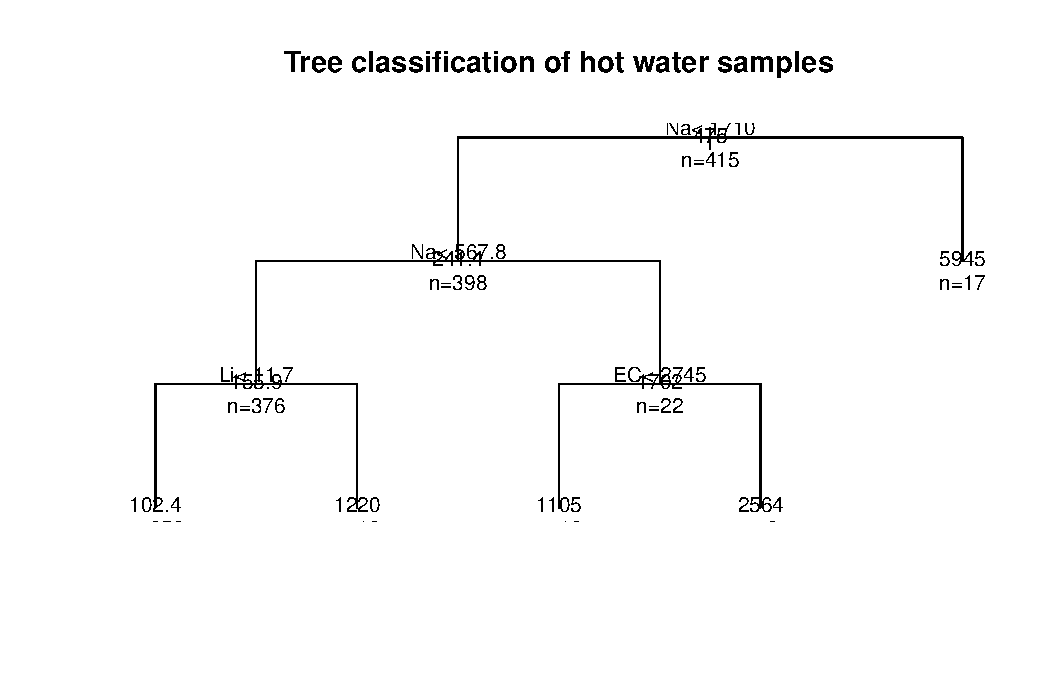
\includegraphics[width=10cm]{treefit_x.pdf}
\end{center}
\caption{ \label{fig:tree} Data classification based on regression tree analysis. }
\end{figure}

\subsection{Cluster analysis and principal component analysis}
The PCA extracts five new sets of variable accounted for 88\% of variation from the original set of 30 variables.(Figure \ref{fig:eigen}), with anomalous data are shown by samples from East Flores and Karaha Bodas. The majority of volcanic samples is  distributed from the center of the plot upwards, while the majority non-volcanic system from the center to the right (Figure \ref{fig:pca}), 

\begin{figure}[h]
\begin{center}
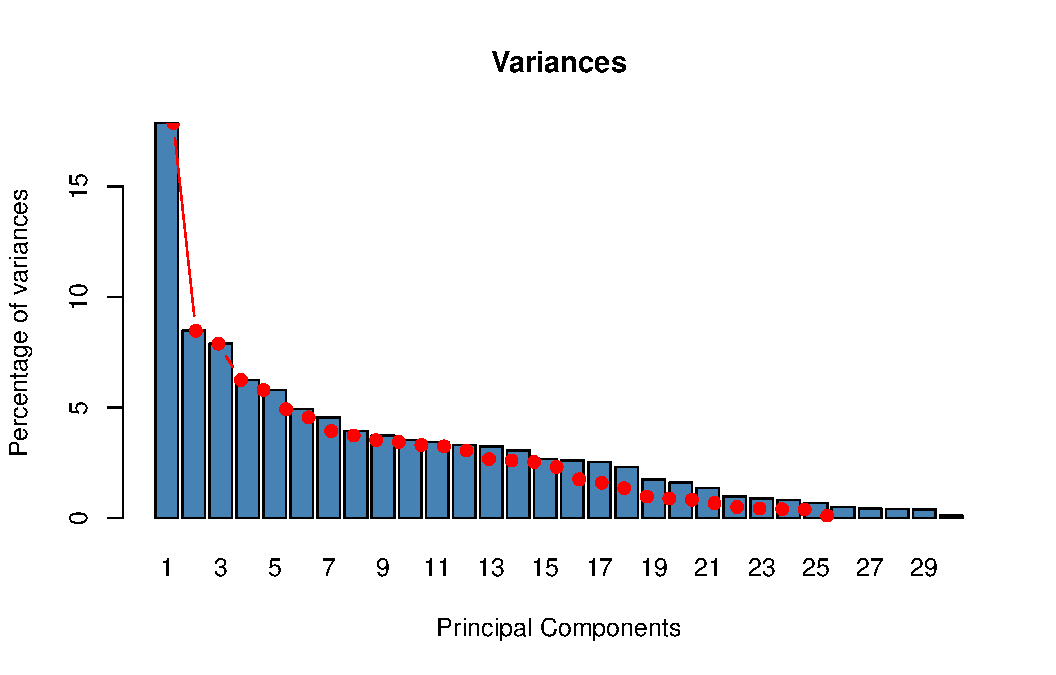
\includegraphics[width=10cm]{eigen_x.pdf}
\end{center}
\caption{ \label{fig:eigen} Eigenvalues from PCA. }
\end{figure}

\begin{figure}[h]
\begin{center}
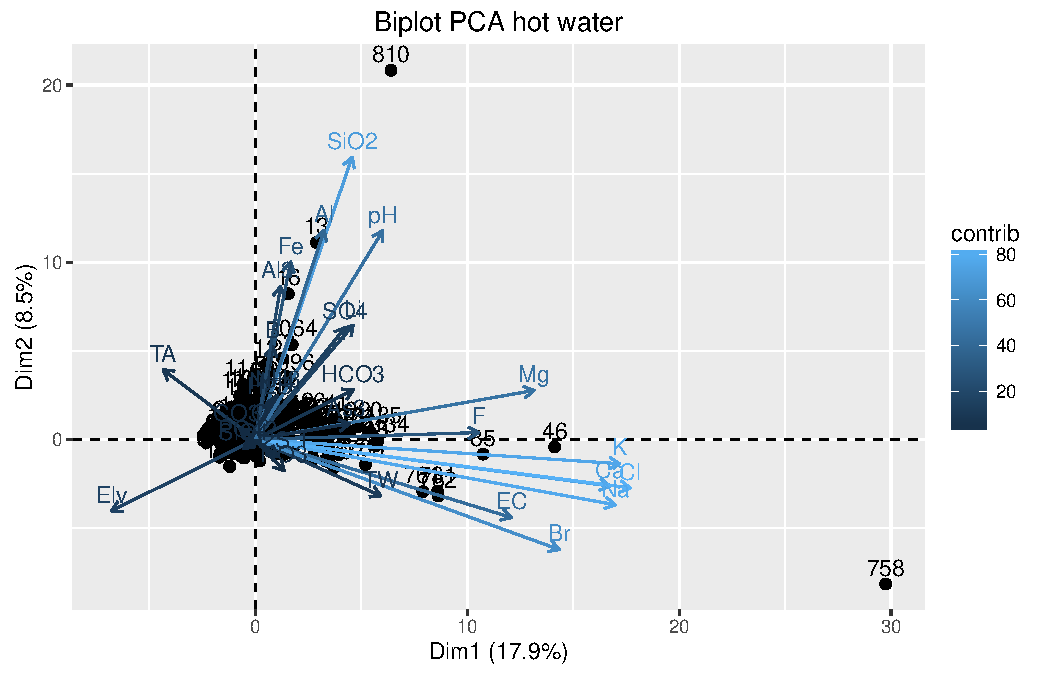
\includegraphics[width=10cm]{pca_x.pdf}
\end{center}
\caption{ \label{fig:pca} Biplot from PCA. }
\end{figure}

We identify three major clusters based on the dendogram: cluster 1 (pure hot water), which is divided into 1a volcanic system and 1b non-volcanic system, cluster 2 (mixing water), and cluster 3 (cold-meteoric water). Mixing processes occur in each system due to the high rainfall (Figure \ref{fig:cluster}).

\begin{figure}[h]
\begin{center}
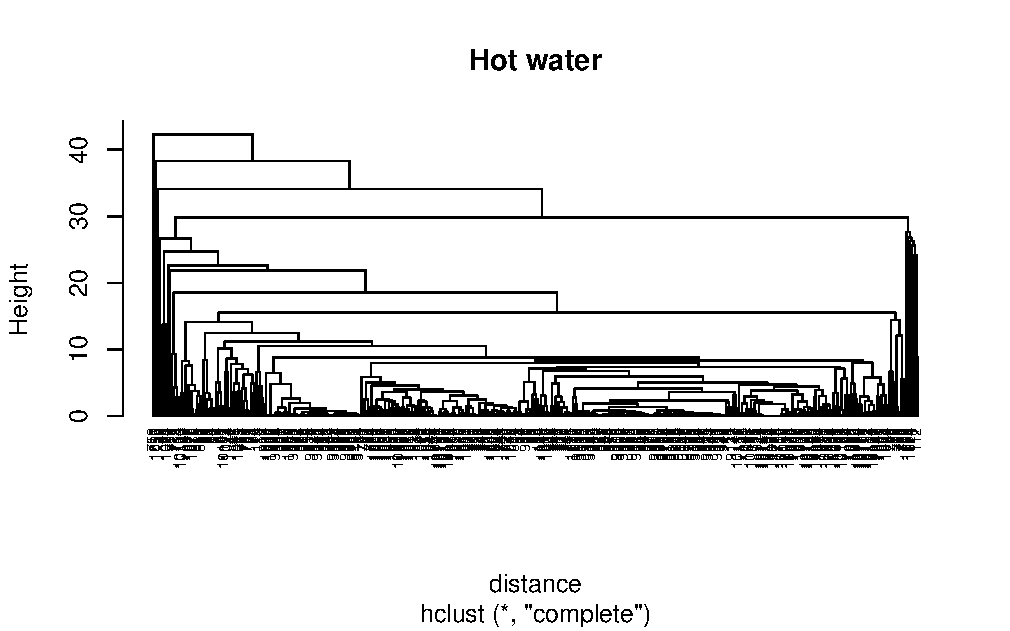
\includegraphics[width=10cm]{cluster_x.pdf}
\end{center}
\caption{ \label{fig:cluster} Dendogram from cluster analysis. }
\end{figure}

After evaluating the results we are not be able to draw a firm conclusion at this moment. We need to sort out the dataset based on the heterogeneity. 

 
\section{References}

\begin{enumerate}

\item Agustin, A., Irawan, D.E., Susanto, A., Herdianita, N.R., 2015. Application of Geochemical Methods in Geothermal Exploration in Indonesia: a Literature Review (Part 1), PROCEEDINGS, 3rd IIGW ITB, Bandung, Indonesia.

\item ath, G. De’, Fabricius, K.E., 2000. Classification and regression trees: a powerful yet simple technique for ecological data analysis. Ecology 81, 3178–3192.

\item Bronto, S., 2006. Fasies gunung api dan aplikasinya. Indones. J. Geosci. 1, 59–71.

\item Chen, K., Jiao, J.J., Huang, J., Huang, R., 2007. Multivariate statistical evaluation of trace elements in groundwater in a coastal area in Shenzhen, China. Environ. Pollut. 147, 771–780.

\item Darmawan, I.G.B., Setijadji, L.D., Wintolo, D., 2015. Geology and Geothermal System in Rajabasa Volcano South Lampung Regency, Indonesia (Approach to Field Observations, Water Geochemistry and Magnetic Methods). Geology 19, 25.

\item Faraway, J.J., 2005. Extending the linear model with R: generalized linear, mixed effects and nonparametric regression models. CRC press.

\item Fauzi, A., 2015. Geothermal resources and reserves in Indonesia: an updated revision. Geotherm. Energy Sci. 3, 1–6. doi:10.5194/gtes-3-1-2015

\item Fitzpatrick, M.L., Long, D.T., Pijanowski, B.C., 2007. Exploring the effects of urban and agricultural land use on surface water chemistry, across a regional watershed, using multivariate statistics. Appl. Geochem. 22, 1825–1840.

\item Gio, Prana Ugiana, Rosmaini, Elly, 2015. Belajar olah data dengan piranti lunak statistik. USU Press, Medan.

\item Gregor, J., Garrett, N., Gilpin, B., Randall, C., Saunders, D., 2002. Use of classification and regression tree (CART) analysis with chemical faecal indicators to determine sources of contamination. N. Z. J. Mar. Freshw. Res. 36, 387–398.

\item Irawan, D.E.., Puradimaja, D.J.., Notosiswoyo, S.., Soemintadiredja, P.., 2009. Hydrogeochemistry of volcanic hydrogeology based on cluster analysis of Mount Ciremai, West Java, Indonesia. J. Hydrol. 376, 221–234.

\item King, A.C., Raiber, M., Cox, M.E., 2014. Multivariate statistical analysis of hydrochemical data to assess alluvial aquifer–stream connectivity during drought and flood: Cressbrook Creek, southeast Queensland, Australia. Hydrogeol. J. 22, 481–500. doi:10.1007/s10040-013-1057-1

\item Kuhn, M., 2008. Building predictive models in R using the caret package. J. Stat. Softw. 28, 1–26.

\item Lewis, R.J., 2000. An introduction to classification and regression tree (CART) analysis, in: Annual Meeting of the Society for Academic Emergency Medicine in San Francisco, California. pp. 1–14.

\item Loh, W.-Y., 2011. Classification and regression trees. Wiley Interdiscip. Rev. Data Min. Knowl. Discov. 1, 14–23.

\item Manalu, P., 1988. Geothermal development in Indonesia. Geothermics 17, 415 – 420. doi:http://dx.doi.org/10.1016/0375-6505(88)90070-3

\item Ritzi, R.W., Wright, S.L., Mann, B., Chen, M., 1993. Analysis of temporal variability in hydrogeochemical data used for multivariate analyses. Groundwater 31, 221–229.

\item Rothwell, J.J., Futter, M.N., Dise, N.B., 2008. A classification and regression tree model of controls on dissolved inorganic nitrogen leaching from European forests. Environ. Pollut. 156, 544–552.

\item Seyhan, E., Griend, A.A.V.D., Engelen, G.B., 1985. Multivariate Analysis and Interpretation of the Hydrochemistry of a Dolomitic Reef Aquifer, Northern Italy. Water Resour. Res. 21, 1010–1024. doi:http://dx.doi.org/10.1029/wr021i007p01010

\item Smillie, A., Satar, S., Saptadji, N., Aminzadeh, F., Setianingsih, R., n.d. Capacity Building in the Geothermal Sector in Indonesia, a Unique Collaboration.

\end{enumerate}

%% Note: use of BibTeX als works!!

%\bibliographystyle{plain}
%\begin{thebibliography}{1}

%\bibitem{Flusser:Suk:93}
%J.~Flusser and T.~Suk.
%\newblock Pattern recognition by affine moment invariants.
%\newblock {\em Pattern Recognition}, 26:167--174, 1993.

%\bibitem{Hu:62}
%M.~K. Hu.
%\newblock Visual pattern recognition by moment invariants.
%\newblock {\em IRE Transactions on Information Theory}, IT-8:179--187, 1962.

%\bibitem{maragos89:_patter}
%P.~Maragos.
%%\newblock Pattern spectrum and multiscale shape representation.
%\newblock {\em IEEE Trans. Patt. Anal. Mach. Intell.}, 11:701--715, 1989.

%\bibitem{Meijster:Wilkinson:PAMI}
%A.~Meijster and M.~H.~F. Wilkinson.
%\newblock A comparison of algorithms for connected set openings and closings.
%\newblock {\em IEEE Trans. Patt. Anal. Mach. Intell.}, 24(4):484--494, 2002.

%\bibitem{Nacken:thesis}
%P.~F.~M. Nacken.
%\newblock {\em Image Analysis Methods Based on Hierarchies of Graphs and
%  Multi-Scale Mathematical Morphology}.
%\newblock PhD thesis, University of Amsterdam, Amsterdam, The Netherlands,
%  1994.

%\end{thebibliography}

\end{multicols}

\end{document}